\section{\system{}: System Design}
In light of the results presented in the previous section, we see that an 
overlay network can significantly help a client avoid any given country.  
Therefore, we have designed and developed a system, \system{}, that allows users 
to route around a specified country.

\subsection{Architecture}

There are three main components to \system{}: the oracle, the relays, and the 
clients.  Figure \ref{fig:arch} shows which components communicate with 
eachother and in which direction the communication occurs.  The relays run as 
proxy servers in addition to periodically measuring paths from itself to the 
top domains that a given client might access and the paths from itself to a 
location near the given client.  The oracle periodically fetches the 
relay-to-domain paths, as well as calculating various other paths.  Using a RIPE
 Atlas probe in the same country as a client, the oracle can measure: the paths
 from a location close to the client (which we will refer to as the client from 
now on) to the relays, and the paths from the client to the domains.  Once these
 paths are mapped to the country level, the oracle can generate and publish a 
Proxy Autoconfiguration (PAC) file, which allows the client to easily configure 
they're browser to use \system{} by specifying the URL where the PAC file resides.
  The PAC file specifies which proxy to use when accessing a specific domain, 
or whether or not to use any proxy.  More detail are discussed in the following 
sections.

\begin{figure}[t]
\centering
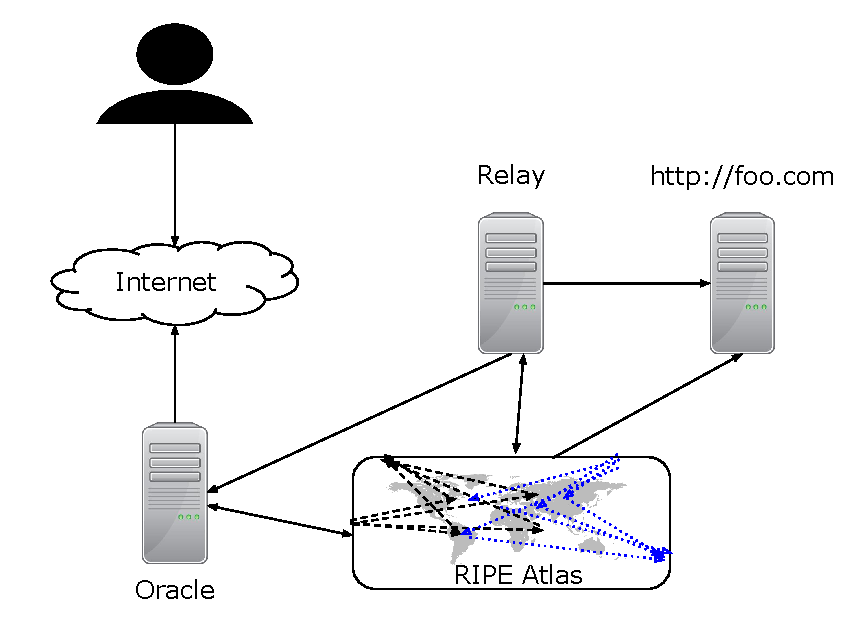
\includegraphics[width=.5\textwidth]{architecture}
\caption{\system{} architecture.}
\label{fig:arch}
\end{figure}

\subsection{Goals}
Here we highlight the main goals of \system{}, as well as challenges that are out 
of the scope of this work.

{\bf Foreign Country Avoidance.}  The primary goal of \system{} is to avoid a given
 country when accessing web content.  \system{} should provide clients a way to 
route around a specified country, while still being able to access the desired 
domain.

{\bf Usability.} \system{} should be designed in a way that is accessible to and 
easy to use by clients around the world.  It should require as little effort by 
the client as possible.

{\bf Scalability.}  This country avoidance system should be able to scale to 
large numbers of users.  Therefore, \system{} should be able to handle the addition
 of relays, as well as be cost-effective in terms of resources required.

{\bf Non-goals.}  There are some challenges that \system{} does not attempt to 
solve.  The system does not address the notion of anonymity; it routes are 
countries (for reasons such as avoiding mass surveillance), but it does not 
attempt to keep users anonymous.  

Additionally, \system{} does not solve the problem of domestic surveillance (for 
example, a client in the United States attempting to avoid surveillance by the 
United States).  This is a challenging problem, and asks for future research, 
but this is out of the scope of our work.

\subsection{Calculating Paths}
Given a set of relays that function as proxy servers, it is challenging to 
measure the necessary country-level paths that will allow the system to specify 
which proxy to use for a given domain.  Here we explain which paths we measure, 
and how and where they are measured.  All of the paths are measured using {\tt 
traceroute}, which is then mapped to the country level using the same methods as 
described in Section \ref{datasets} and shown in Figure 
\ref{fig:analysis_pipeline}.  The paths we measure are the: forward paths from 
the client to each relay, forward paths from each relay to each domain, forward 
paths from the client to each domain, and reverse paths from each relay to the 
client.  The one portion of a path that we cannot measure is the reverse path 
from each domain to each relay; we cannot measure this because we have no 
vantage point at or near the domain from which to run {\tt traceroute}.

{\bf Client to Relay Paths.} As previously mentioned, one of the goals of the 
system is usability, and therefore, the client should not have to perform 
almost any actions.  To keep the client from having to download any software, 
the paths from clients to relays are measured using RIPE Atlas probes.  A probe 
is selected from a geographically close location to the client (i.e. the same 
country), and the oracle triggers the probe to run {\tt traceroute} measurements 
to each relay in the system.  After collecting the responses, the oracle maps 
the IP-level paths to country-level paths and stores the results.

{\bf Relay to Client Paths.} The relays are set up with software to run 
{\tt traceroute} measurements to the IP addresses of RIPE Atlas probes, which 
represent clients.  They then map the responses to country-level paths, and 
store them locally; the oracle will fetch these paths from each relay. 

{\bf Relay to Server Paths.} The software on the relays also runs {\tt 
traceroute} measurements to each domain.  Similar to the paths to clients, these 
are mapped to country-level paths, stored, and then fetched by the oracle.

{\bf Client to Server Paths.} In the case that a path from a client to a 
domain does not pass through the country specified to avoid {\it by default}, 
then none of the proxies should be used.  If a proxy is used, then it may 
actually be causing the path to traverse more countries (unnecessarily).  These 
paths are measured using the RIPE Atlas probes in similar locations as the 
clients, and the oracle triggers {\tt traceroute} measurements to be run from 
them to each of the domains.  The results are converted to country-level paths 
and stored on the oracle.  

Each of these types of paths must be computed initially, but also re-computed 
as paths may change.  To our knowledge, there has not been any previous work 
on how often country-level paths change; prior work has explored how often 
AS-level paths change.  To measure how often country-level paths change, we 
computed the paths from relays to domains once every two hours and once every 
hour.  On average, the path to X domains changed every two hours, and the path 
to Y domains changed every one hour.  As it takes approximately 30 minutes to 
compute all paths, \system{} re-computes the paths every one hour to incorporate 
the most recent country-level paths in the system.

\begin{figure}[t]
\centering
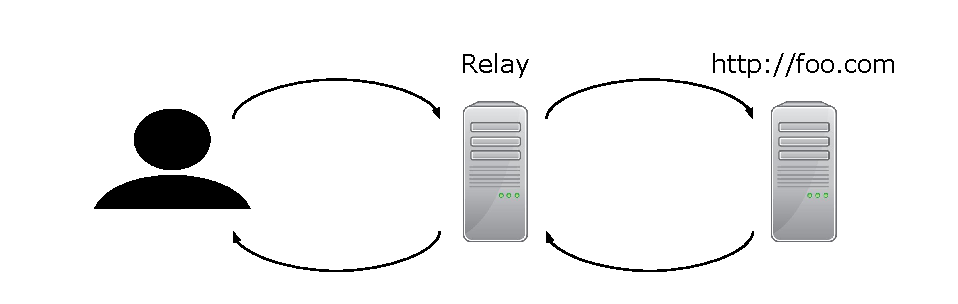
\includegraphics[width=.5\textwidth]{client_to_relay_to_domain}
\caption{The path of a web request through a \system{} relay, to the domain, and back.}
\label{fig:path_components}
\end{figure}

As seen in Figure \ref{fig:path_components}, there are four path components 
when a client accesses web content through \system{}.  The system measures three 
out of the four paths; the reverse path from the domains (servers) to the relays 
is challenging to measure due to a lack of vantage points.  Despite not 
calculating all of the country-level path components, we can show that the 
country a client is attempting to avoid cannot conduct traffic analysis attacks 
on the traffic because {\it at most} the attacker is only on the reverse path 
from the server to the relay.  An attacker would need at least two path 
components to perform traffic analysis. 

\subsection{Multiplexing Between Relays}
\label{multiplex}
After measuring and aggregating the country-level paths, the oracle decides 
which relay to use when accessing specific domains from a specific client 
location.  This decision follows three sequential steps:

\begin{enumerate}
\item If the default path from the client to the domain does not pass through 
the specified country, then do not use any of the relays. Otherwise, continue 
to the next step.
\item For all the paths from the client to the relays, select usable relays 
such that the path does not contain the specified country.
\item From the set of usable relays, if there is a path from a 
usable relay to the domain that does not include the specified country, then 
use that relay for that domain.
\item If there is no path from the client through any of the relays to the domain 
that does not pass through the specified country, then select the relay 
that provides the most avoidance (measured by how many other domains it has 
a path to that avoid the specified country).
\end{enumerate}

The oracle applies this decision process to each domain, and generates a PAC 
file, which specifies which domains should be accessed through which proxy.  A 
sample PAC file is shown in Listing \ref{lst:pac}; in this example, proxy 
1.2.3.4:3128 should be used when accessing {\tt www.google.com}, but proxy 
5.6.7.8:3128 should be used when accessing {\tt www.twitter.com}.  Once the PAC 
file is generated based on the decision chain above, it is published to a URL 
of the format $<$client\_country$>$\_$<$country\_to\_avoid$>$\_pac.pac.  The client 
simply uses this URL to specify their proxy configuration.

\lstinputlisting[label={lst:pac}, language=JavaScript, frame=single, basicstyle=\footnotesize, caption={An example PAC file.}]{example_pac.pac}

As paths are re-computed every hour, the PAC file is also re-computed and 
published every hour.

\subsection{Scaling the System}
In addition to usability, another goal of \system{} is scalability.  The system 
must support increasing numbers of users.  

{\bf Adding Relays.} As the number of clients increase, their locations may be 
extremely diverse. This calls for a geographically diverse set of relays, as 
well as a set of relays that can grow with the number of clients (duplicates in 
the same locations used to balance the load).  \system{} is 
designed in a modular way, and therefore, adding relays is quick, easy, and 
simple.  To add a relay, the system operator must set up a machine as a proxy 
server, install the \system{} relay software, and update the oracle's list of 
relays.  From that point forward, paths will be computed to and from the new 
relay, and clients will be using it as a proxy.  

{\bf Adding Oracles.} As the number of clients increase, it is possible that a 
single oracle can not tolerate the computation or storage space necessary for 
all clients.  Adding an oracle is a matter of installing the oracle software on 
a different machine, and specifying the client locations handled by that oracle 
(for example, oracle 1 handles all clients in North America and Europe, and 
oracle 2 handles all clients elsewhere).  Both oracles will publish the PAC files 
to the same server, which causes no changes for the client.

\subsection{Fault Tolerance}
\system{} is resilient to crashed system components, such as a crashed relay or 
oracle.  

{\bf Failed Relay.} If a relay becomes unresponsive, this issue is handled by 
the PAC file.  The PAC file allows the oracle to specify multiple proxies in 
a sequential order, such that if the the first proxy fails, then the second 
proxy is used (and so on).  This feature can be used to specify all of the 
relays that have a path to the domain.  And future work can include relay 
replicas that can be used in the case that a relay crashes.

{\bf Failed Oracle.} If an oracle crashes, it could trigger a backup oracle 
to re-compute the PAC files periodically.  This is a simple solution because 
the oracles do not need to convey any information among each other, and therefore, 
no information is lost.  We leave the implementation of backup oracles as future 
work.

It is worth noting that without backup oracles, clients can still use the system 
when the oracle fails.  The clients will simply be using stale paths, which are 
likely to be the same original paths, but not always.  

\subsection{Additional Features}
We have implemented \system{} as discussed above, but the system design allows for 
additional features to be added in the future to enhance the system.

{\bf Privacy-preserving features at relay.}  Additional features can be 
implemented at the relay to help preserve client privacy.  Such an example would 
be to use the relay as a mix, or to send out fake traffic to confuse an 
attacker that may be trying to perform traffic analysis at the relay.

{\bf Load balancing and congestion control.} The oracle could add additional 
steps in the decision chain introduced in Section \ref{multiplex} that take 
into account relay and path loads.  For example, if multiple relays provide 
a path to a domain that do not traverse the specified country, then the 
decision between the usable proxies could be determined based on current relay 
load.

{\bf Optimized performance.} In addition to load balancing purposes, the oracle 
could make relay decisions based on performance.  For example, if there are 
multiple usable relays, the decision could be made on how much time it would 
take to access the content from each of the relays.

{\bf Precise path re-computation.}  Our current implementation of \system{} 
re-computes all paths once per hour.  This could be optimized to only re-compute 
paths when necessary.  For example, a BGP monitoring system could be implemented 
that alerts the oracle to a path change that affects any path currently in 
the system.  This could decrease the cost and computation of the system.
